\section{Design of \tachyon}



\subsection{Overview of \tachyon and Challenges}

\begin{figure}
  \centering
  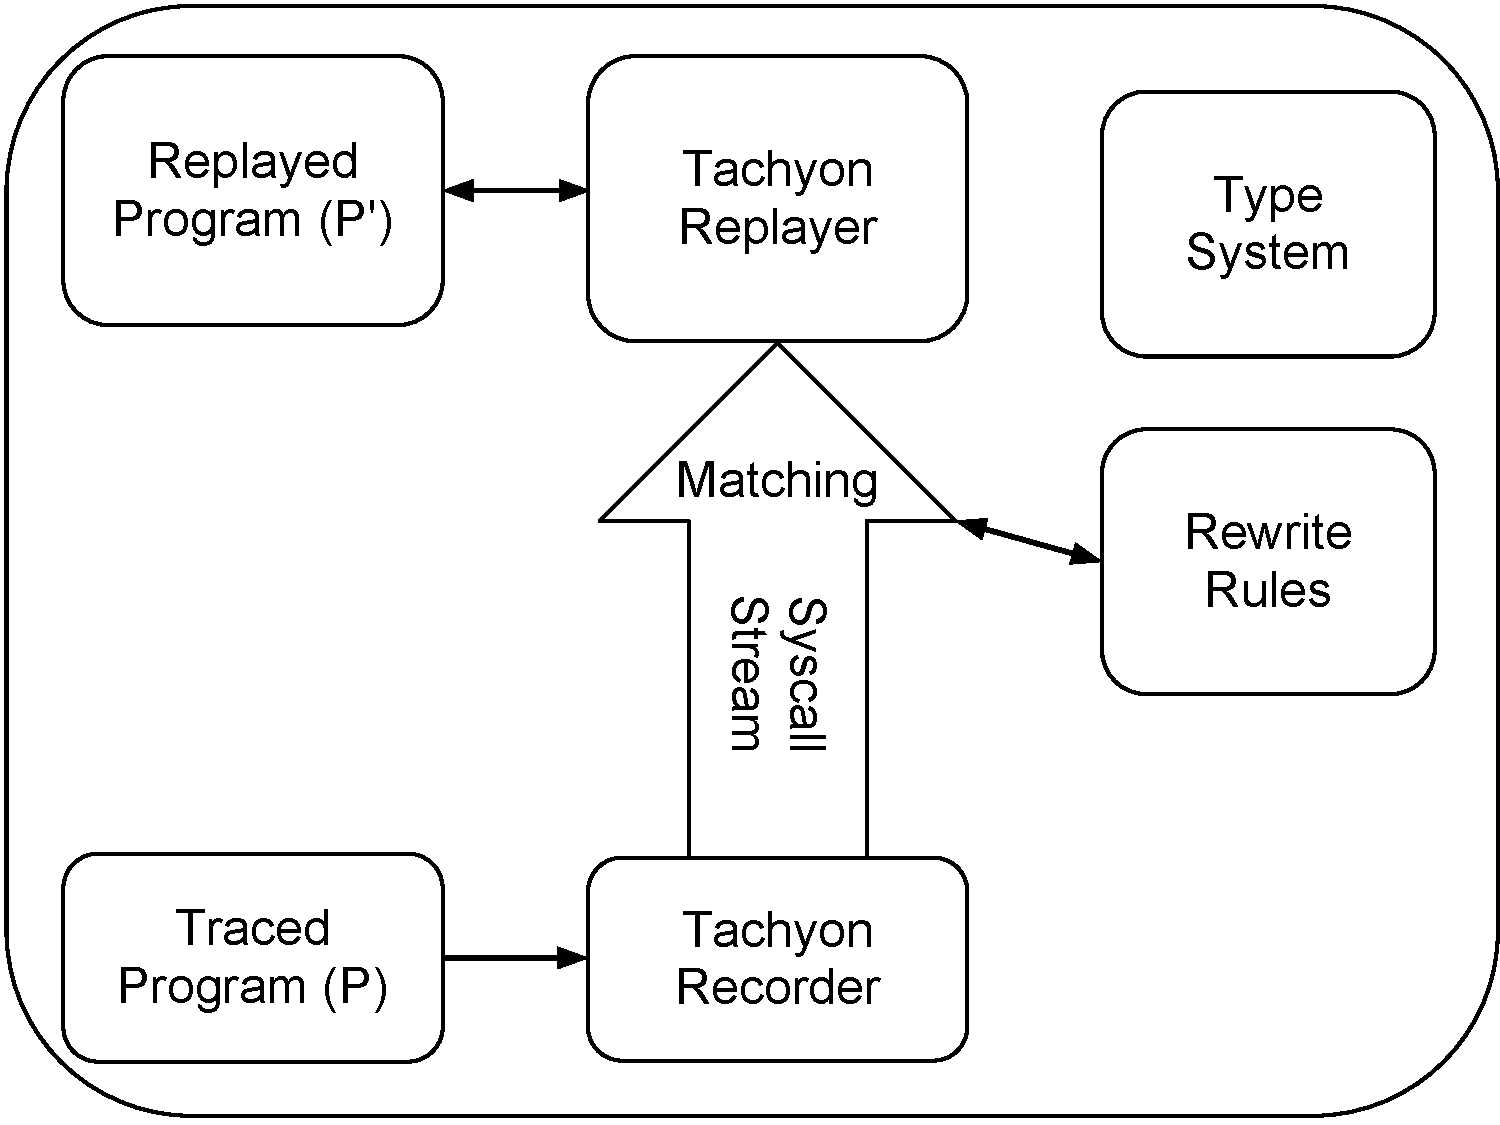
\includegraphics[scale=0.5]{tachyon/TachyonDiagram.pdf}
  \caption{Tachyon System Overview}
  \label{tach:fig:system}
\end{figure}

The overall architecture of \tachyon is shown in
Figure~\ref{tach:fig:system}.
We will refer to the program running
live  as $\patched$ (e.g., the patched program) and the program running
in-tandem with simulated syscalls as $\unpatched$ (e.g., the unpatched
program).  \tachyon is a user-land program that utilizes the Linux
ptrace facility to interpose on syscalls issued by $\patched$ and
$\unpatched$.  Like replay schemes, \tachyon has a recorder and a
replay module. The recorder records the stream of system calls
issued by $\patched$ and outputs a stream of tuples
$\tuple{C}{\vec{I}}{\vec{O}}$ where $C$ is the system call number,
$\vec{I}$ is a list of inputs to the system call, and $\vec{O}$ is a
list of outputs.  The replay module interposes on $\unpatched$, and
for each syscall $C$ with arguments $\vec{I}$ made by $\unpatched$,
simulates the OS by returning $\vec{O}$.

\begin{lstlisting}[float,caption={Example patch},label={tach:lst:example}]
-int fd = open("/tmp/fileA", O_RDONLY);
+int fd = open("/tmp/fileB", O_RDWR);
-int *storage = malloc(...);
-/* ... Do some processing with storage..  */
+fstat(fd, statBuf);
 char* incoming = malloc(chunksize);
 ssize_t size = read(fd, incoming, chunksize);
 if (size != -1)
   write(fdOut, incoming, size);
\end{lstlisting}

Consider the example shown in Listing~\ref{tach:lst:example}, with the
patch difference being displayed in diff style with full context. The first
edit changes the file opened from \texttt{/tmp/fileA} to
\texttt{/tmp/fileB}. The next few edits remove an unneeded call to
{\tt malloc}, and add {\tt fstat}.  The rest of the program is the
same. Note that since a {\tt malloc} call was removed, the returned
memory chunk for {\tt incoming} will be at a different address, even
on systems with a deterministic memory layout.  Overall, this patch
example illustrates three challenges: patches may change arguments to
system calls, may change system calls issued, may change memory
allocation patterns, and any of these changes may have effects on subsequent
execution.

% Essentially, we see here an earlier bit of processing which used an allocation
% was removed, along with an unneeded \texttt{fstat}. The call to \texttt{write}
% emphasizes the challenge of isolation for tandem execution, as a bad program
% would clobber the output of the good program. The change in allocations between
% the two moves the memory layout around, making memory diffing techniques
% ineffective for recording effects, emphasizing the second challenge. Finally,
% the spurious \texttt{fstat} which is dropped in the patch should be accepted,
% showing the need for a system call stream rewriting.


The above challenges motivate three main requirements of live patch
testing as distinguished from a normal replay system. First, instead
of offline replay, a live patch testing solution should be
\emph{online} where $\patched$ produces the syscall stream that
$\unpatched$ should consume.  Second, a live patch tester should not
depend upon pointers because absolute memory addresses may change
between runs. For example, $\unpatched$ and $\patched$ may issue
calls to {\tt malloc} for different amounts or ASLR may be enabled.
Either case prevents patch testing. As a result, we cannot determine
$\vec{O}$ by simply diffing the memory state
before and after a syscall, as in previous syscall replay
schemes~\cite{\allsystemcallreplay}.  Additionally, memory diffing
does not allow us to determine the inputs $\vec{I}$ to system
calls. As a good live patch tester should verify the inputs as well,
we need some way to extract all inputs of a system call. Without a
semantic model, we will be unable to both locate all the relevant
components of the input, and to avoid capturing irrelevant components.
Thus, we need a semantic model of the inputs. Third, since a patch
may remove or add system calls, the live patch testing scheme should
allow for the syscall stream to be rewritten during replay. This can be accounted for by allowing
rewriting of the tuple stream $\tuple{C}{\vec{I}}{\vec{O}}$.  


\subsection{System Calls and Side-Effects}

\tachyon needs to determine what the semantic inputs and outputs
to a syscall are in order to record and replay them.  Specifically, it needs to (1) determine the types of
arguments to a syscall, (2) differentiate input from
output, and (3) pointers from the pointed-to data. While existing C
syscall prototypes are sufficient  for (1), they do not provide enough
information for (2) and (3). Consider the
\texttt{read} syscall declaration:
\begin{lstlisting}
ssize_t read(int fd, void *buf, size_t count);
\end{lstlisting}

This C declaration misses crucial information.  First, it
gives no clue how the void pointer buf works. How big is it? Is it
null-terminated? Are the contents relevant before the call, after, or
both? We need to answer all these questions in order to copy the
appropriate semantic data.  We can see that even the assertion that a
pointer points at some data before or after the system call is not the
case, as with \texttt{sbrk} (pointer points at the end of your address space)
 and \texttt{mmap} (one pointer is only a suggestion). {\tt read} is one of the
simple cases; several syscalls have complicated dependencies between
input and output parameters, as will be discussed later in~\S\ref{tach:sec:types}.

\tachyon addresses the challenges associated with understanding the
semantics of syscalls by adding type annotations, as described in~\S\ref{tach:sec:types}. The \tachyon 
annotation language is a light-weight dependent type system that says
how to parse the inputs and arguments into semantic data at runtime.
These type annotations only need to be written once per system call,
and are portable across systems with the same syscall signatures.

\subsection{Syscall Stream Rewriting}

%\edissue{Maurer: Done. Honestly, I liked cURL better, but I understand trying to have a single example for the section.}

Many patches also change the sequence of syscalls made in addition to
the actual parameters.  Consider Listing~\ref{tach:lst:example}.  The
system call stream when executing the patched program is $\langle ...,
{\tt open}, {\tt fstat}, {\tt read}, {\tt write}, ...\rangle$.
However, the call after {\tt open}  in the unpatched program is {\tt
  read}, not {\tt fstat}.  

%Thus, the two programs have semantically
%different behavior, which we will report as a deviation.



New patched versions often have new system call patterns that cause
the program to behave differently at an IO level. It is not possible
to tell whether a particular change in system call patterns is valid
without a human to validate it. For example, if it turns out the
above code is just shifting a few things around and adding a new
inconsequential call to \texttt{fstat}, then the user may want to
ignore the deviation.  However, the \texttt{fstat} may have been
inserted for security, and a deviation may indicate an attack.  When
opening files in \texttt{/tmp/} a common security practice is to
then call \texttt{fstat} to obtain the user ID and group ID of the
file to make sure they are correct in order to detect race
conditions. \tachyon should report the deviation and halt execution in
such instances. 

Although we cannot automatically decide which deviations matter,
\tachyon does \emph{automate finding deviations}, as well as provide a
mechanism to ignore such deviations when found to continue testing.
The rewriting engine relies upon rules that are created for each
patched program that detail how to handle semantic differences. For
example, if a system administrator decides the above deviation is
inconsequential a rule can be written to ignore the {\tt fstat} call.
Alternatively, patch creators could write such rules and distribute
them with their patches to aid testing.

\subsection{Road Map}
In the rest of this chapter, we first describe the \tachyon type system in detail. We
then discuss how \tachyon rewrites system calls, as well as some
common rules we have found in patches we have tested. We next describe
our implementation and evaluation. We finally discuss several
applications of \tachyon outside automated patch testing.


%%% Local Variables: 
%%% mode: latex
%%% TeX-master: "paper"
%%% End: 
